\chapter{S�ownik u�ytych poj��}
\label{slownik}

\begin{description}
\item[inicjalizacja t�a] proces jednorazowy, w kt�rym na podstawie pewnej ilo�ci ramek i odpowiednich algorytm�w zostaje uzyskany model t�a
\item[generecja t�a] ci�g�y proces aktualizacji wst�pnie zainicjalizowanego modelu  t�a
\item[blok] wydzielona kwadratowa cze�� ramki o~rozmiarach $N*N$, zawieraj�ca opr�cz pikseli informacj� o~wadze superbloku
\item[superblok] grupa 4~s�siaduj�cych ze sob� blok�w, tworz�ca wi�kszy blok(superblok) o~rozmiarach $2N * 2N$
\begin{figure}[ht]
\begin{center}
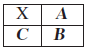
\includegraphics{blok.png}
\caption{Blok X~oraz jego otoczenie, tworz�ce razem z~nim superblok}
\end{center}
\end{figure}  
\item[grupa kandydat�w] utrzymywana dla ka�dego bloku grupa blok�w, kt�re z pewnym prawdopodobie�stwem mog� by� fragmentem t�a
\item[lokalizacja blokowa] - para wsp�rz�dnych (x,y), wyznaczaj�ca miejsce w sekwencji wideo, gdzie znajduje si� dany blok
\end{description}